\section{Background \& related work}
\todo[inline]{%
    \textcite{satyanarayanan2009case}

    Other papers detailing the advantages of Edge computing.

    Next, what applications benefit from the Edge?
    \gls{WCA}! Mention both the main body of work (by Satya et.\ al.) but also other authors out there.
    Main points: prototypes and characterization of system latencies and load.
}

\subsection{Edge computing}

Edge computing is a novel distributed computing paradigm, emerging from a need to overcome the drawbacks of offloading computation and data to the cloud.
Cloud computing, the reigning distributed computing model, allows users to access shared pools of resources such as servers, databases, and applications, over the internet~\cite{gai2012towards}.
These pools of resources are managed in a centralized manner by specialized providers, and users and businesses can access them on-demand, without having to invest in and manage infrastructure of their own.
Providers in turn employ economies of scale, providing these services by deploying massive amounts of computing power and storage capacity in specialized locations known as datacenters~\citationeeded.
These hardware resources are then further compartmentalized through the use of virtualization technologies such as \glspl{VM} and containers~\cite{gai2012towards}.

Through this design, cloud computing affords significant advantages to users.
As services are deployed in a centralized manner accessible over the internet, users can interact with their data and applications from anywhere in the world, from any device.
Thanks to economies of scale and virtualization technologies, the cloud is highly scalable;
services can be scaled simply by spawning more \glspl{VM}.
The specialized nature of cloud providers, the scale of modern datacenters, and the use of virtualization also make the cloud highly reliable.
When hardware fails, recovering is simply a matter of migrating the service container or \gls{VM} to an available compute node~\cite{endo2016high}.

However, the cloud is not suitable for everything, and presents important drawbacks and challenges for latency-sensitive applications.
In order to achieve the necessary economies of scale, cloud datacenters are designed to serve users distributed across vast geographical areas.
These installations are thus often located ``far'' from potential users;
for instance, at the time of writing, \gls{AWS} processes traffic from all of Scandinavia and the Baltic countries through a single datacenter in Stockholm~\cite{awsregions}.
This leads to prohibitively high latencies for both highly interactive immersive applications such as mobile \gls{XR} and for \glspl{CPS} and \glspl{NCS}~\cite{satyanarayanan2009case,varghese2016challenges,shi2016promise}.
The former category requires \emph{motion-to-photon} latencies (i.e.\ time between input capture and feedback) below \SI{60}{\milli\second} for interactions to be perceived as fluid and responsive by the user~\cite{chen2017empirical}; the latter can require sub-\SI{10}{\milli\second} latencies, for instance in the case of vehicular safety systems.
Such latencies are unfeasible to consistently achieve with cloud computing~\cite{dang2021cloudy}.

Current cloud infrastructures are also ill-suited to deal with the bandwidth requirements of the \gls{IOT} and of mobile computing.
As smart devices, appliances, and sensors become more and more ubiquitous, the network architectures of modern datacenters face significant challenges to deal with the massively increasing volume of traffic~\cite{shi2016edge,wang2019towards}.

\begin{figure}
    \centering
    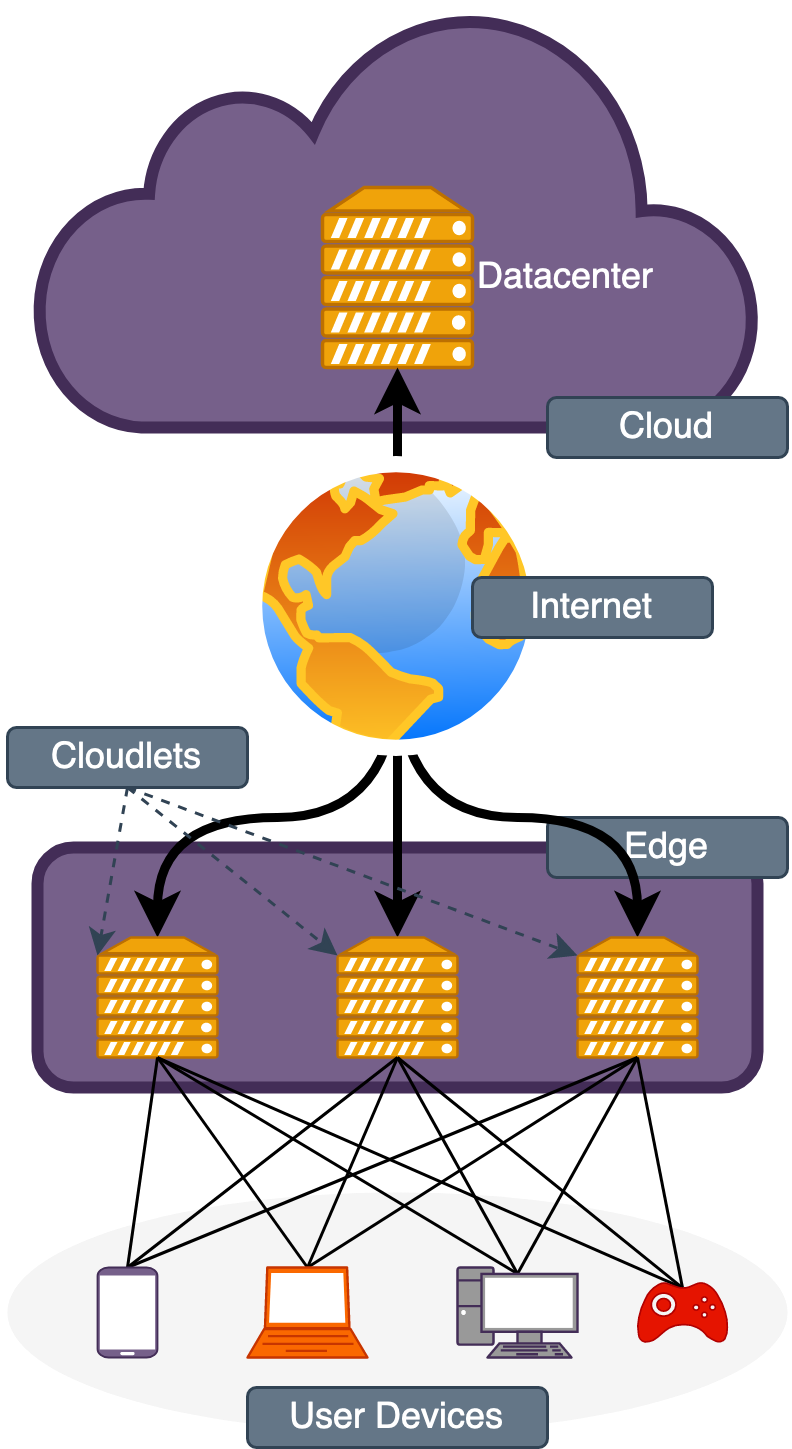
\includegraphics[height=30em]{Figs/edgecomputing}
    \caption{%
        Conceptual design of edge computing.
        Micro-clouds (known as ``cloudlets''~\cite{satyanarayanan2009case}) are placed a at the edge of the network, a few hops away from end users.
        In other words, these cloudlets are located between users and the internet and the cloud.
    }\label{fig:edgecomputing}
\end{figure}

Edge computing, emerges as a potential answer to these challenges~\cite{satyanarayanan2009case,shi2016promise,shi2016edge,varghese2016challenges,satyanarayanan2017emergence,bittmann2017edge,wang2019towards}.
This term refers to a novel distributed computing paradigm, complementary to cloud computing, which tackles the challenges of the cloud by moving computation closer to where it is needed.
Instead of offloading computation to a datacenter potentially thousands of kilometers away, in edge computing it is offloaded to a micro-datacenter --- a \emph{cloudlet}~\cite{satyanarayanan2009case} --- at the \emph{edge} of the network.
These coudlets feature most of the key characteristics of cloud datacenters, such as multi-tenancy, virtualization of computing resources, virtually unrestricted access to energy, as well as limited scalability, one or two hops away from the user (see \cref{fig:edgecomputing})

The architecture of edge computing offers several advantages.
Thanks to their proximity to users, cloudlets can serve highly latency-sensitive and resource-intensive applications with extremely low latencies while still providing orders of magnitude more computing and energy resources than those present on mobile and wearable devices.
Mobile \gls{XR}, such as \gls{WCA}~\cite{ha2014towards,chen2018application,wang2020scaling,chen2017empirical,chen2018application}, and 5G-enabled \glspl{CPS} and \glspl{NCS}~\cite{sasaki2016vehicle,wang2018bandwidth,wan2020efficient} are uniquely poised to take advantage of these characteristic of edge computing.
By processing and aggregating data closer to where its needed, cloudlets can also drastically reduce the amount of traffic going to cloud datacenters.
Cloudlets also present opportunities for increased data security, privacy, and integrity, by keeping it geographically close to its origin and by allowing for anonymization through denaturing and local aggregation before offloading to cloud services~\cite{satyanarayanan2017emergence}.

\todo[inline]{Transition to talk about research and tools for Edge computing research.}

\subsection{\glsfmtlong{WCA}}
\glsreset{WCA}

There is increasing interest from academia and industry in a novel category of wearable and mobile immersive applications called \gls{WCA}~\cite{ha2014towards,chen2018application,chen2015early,belletier2021wearable,chen2017empirical,wang2020scaling,chatzopoulos2017hyperion}
They represent a particular class of \gls{AR} applications, aiming to amplify human cognition in both day-to-day tasks and professional settings.
\glspl{WCA} operate in a mode analogous to how \gls{GPS} navigation systems guide drivers, by seamlessly providing relevant instructions and feedback relating to the current task at hand and staying out of the way of the user when guidance is not required.
These systems were originally inspired by assistive use cases for people suffering from some form of cognitive decline due to aging, illness, or traumatic brain injury~\cite{ha2014towards,satyanarayanan2019augmenting}.
More recently, their scope has been expanded to include a broader range of use cases, including complex assembly tasks~\cite{chen2017empirical,chen2018application,wang2020scaling,wang2019towards,ha2014towards}.
Non-wearable cognitive assistance systems for assembly tasks have already been proven to be valuable tools in the industrial workplace~\cite{funk2015cognitive,gorecky2011cognito}, and it is understood that the detethering of these system for their use in wearable scenarios opens up a multitude of possibilities.
\todo[inline]{Develop a bit further. Talk about more reactive setups like ping pong too.}

\begin{figure}
    \centering
    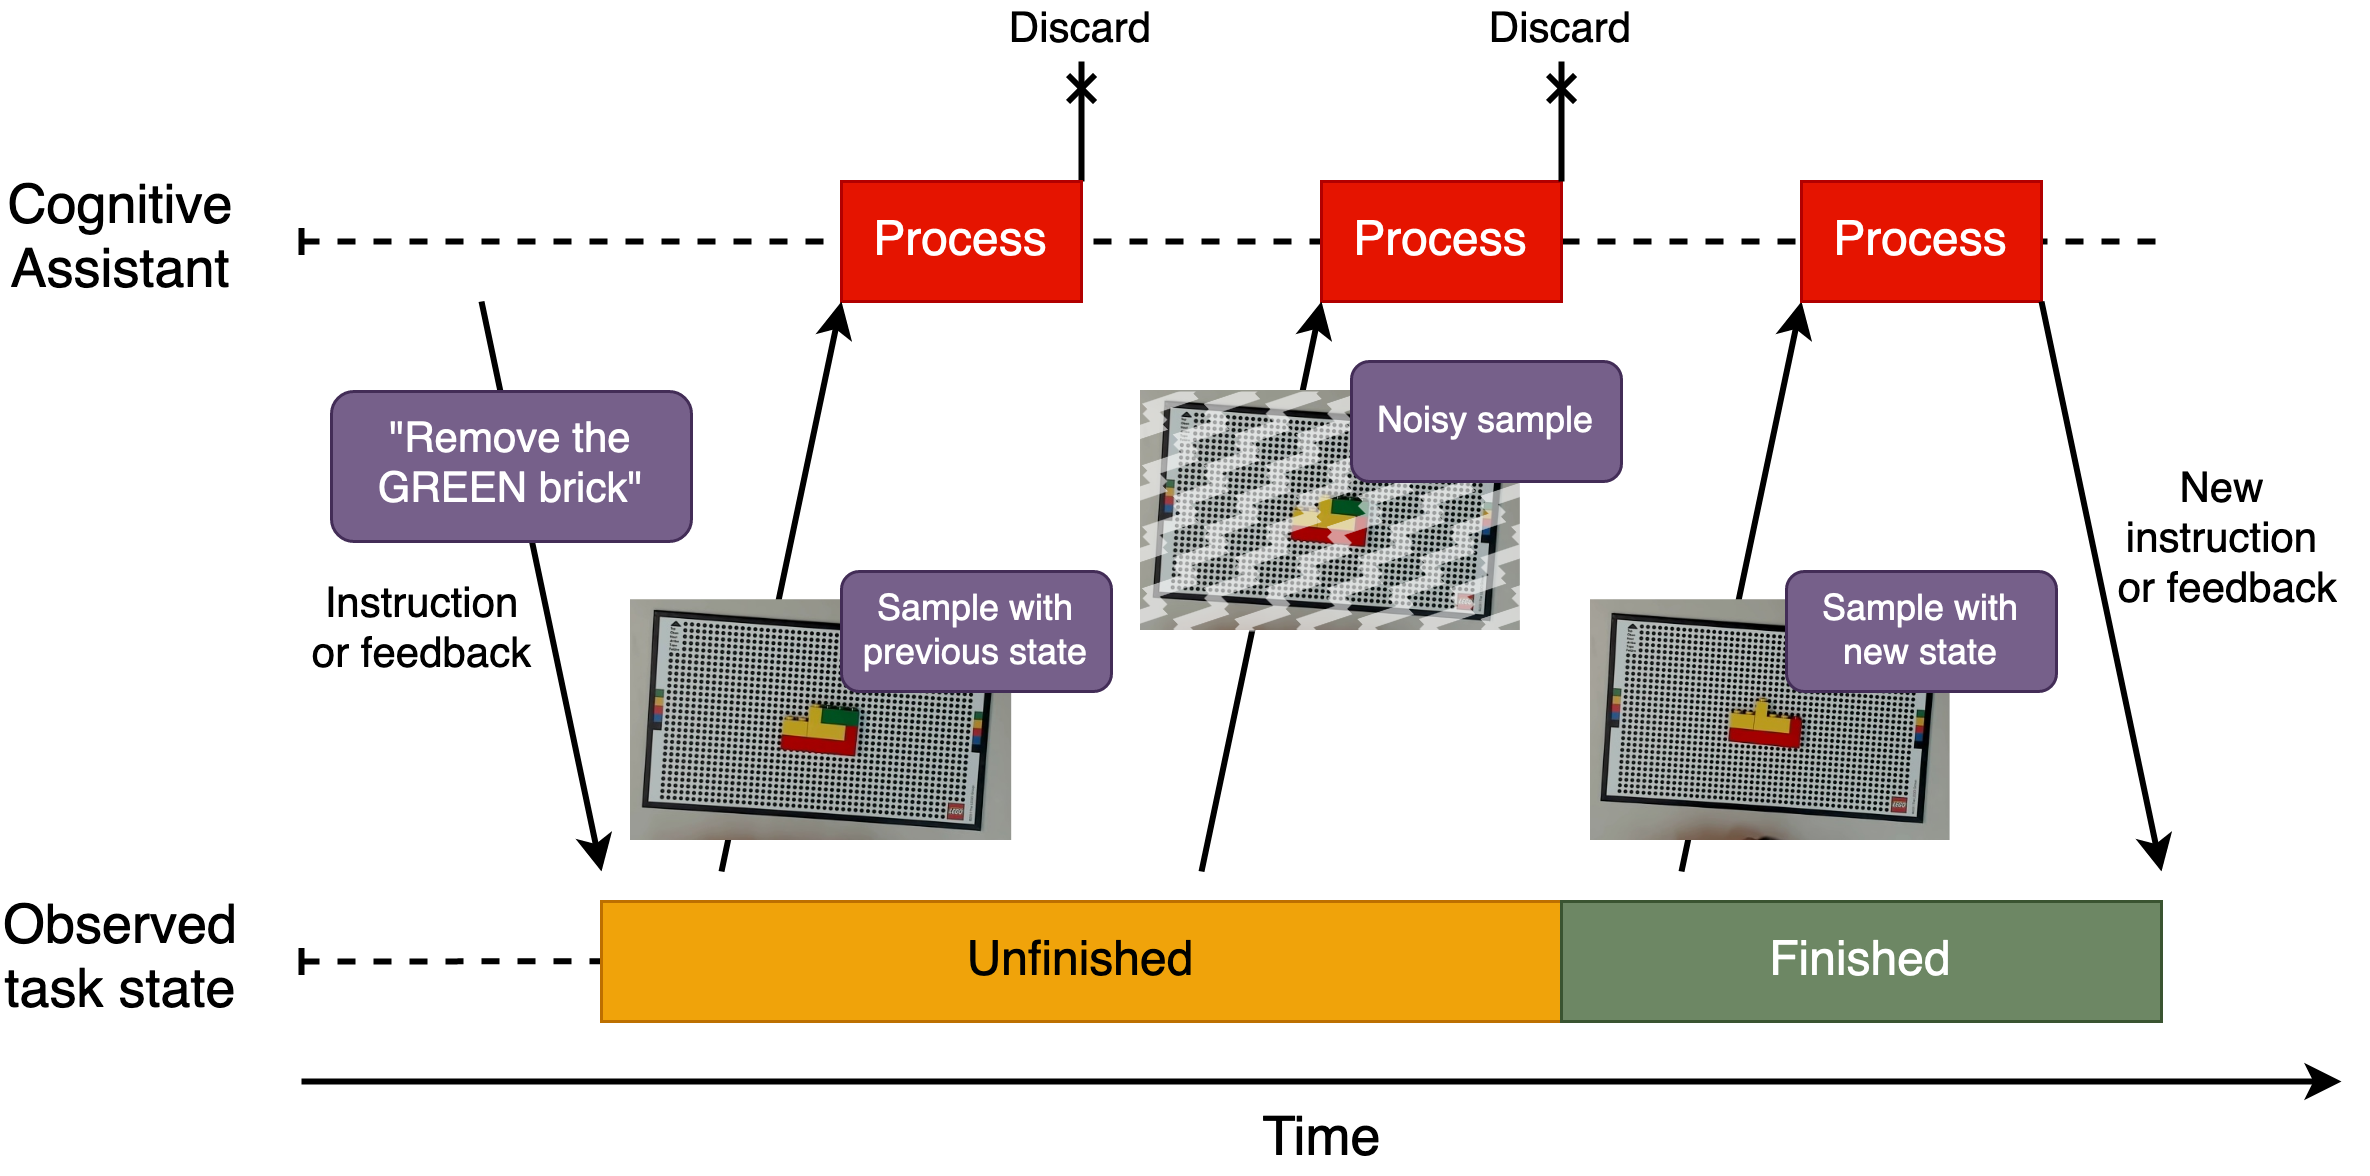
\includegraphics[width=.9\textwidth]{Figs/wca_state}
    \caption{%
        Mode of operation of \gls{WCA} applications.
        The assistant continuously samples the state of the monitored task, and provides appropriate feedback once a state change has been detected.
        Samples that do not result in feedback are silently discarded.
    }\label{fig:wca}
\end{figure}

We identify a number of defining characteristics of \gls{WCA}.
One, and as the name implies, \glspl{WCA} are available whenever the user requires them, without being tethered to a particular physical location;
they are pervasive and mobile~\cite{ha2014towards}.

Next, interaction with \glspl{WCA} is immersive and seamless.
As mentioned above, \glspl{WCA} operate in a manner similar to \gls{GPS} guidance systems.
Through the use of sensors (most commonly video inputs), the application follows the progress of the task in realtime by continuously sampling the state of the physical system.
The input is then parsed to an internal symbolic representation of the state of the task, and whenever a change of state is detected the application provides appropriate feedback or instructions to the user.
Feedback can be in the form of text, images, video, and/or audio, and guides the user towards the next desired system state.
If no change in state is detected, the application remains silent and out-of-the-way of the user;
in other words, samples which capture an intermediate or unfinished state, or simply noise are silently discarded.
\Cref{fig:wca} illustrates this mode of operation in a \gls{WCA} guiding a user to manipulate a structure composed of LEGO bricks.
Assistants should be able to analyze the current context and automatically provide relevant feedback without explicit commands from the user.
\gls{WCA} is expected to operate much like a human assistant would, by observing the performance of the user and offering guidance proactively.

Note that this mode interaction implies seamless integration of the application with the context of the user and the real world.
The user does not trigger an update explicitly at any point, leading to one of the key characteristics of \gls{WCA}.
The only points in time at which a user can consciously notice and interact with the application is whenever they are \emph{expecting} feedback.
An important corollary of this is that these are therefore the \emph{only} points in time at which users can notice changes in system responsiveness.

Finally, feedback in \gls{WCA} systems should be provided ``quickly'' (relative to the task at hand) to the user.
This goes hand in hand with the previous characteristic of seamless interaction, as users will have expectations of constant and immediate feedback as they interact with the system.
As is the case for most \gls{XR} applications, delayed feedback in \gls{WCA} can have severe negative consequences for the quality of the user experience.
Depending on the task, these consequences can range from simply distracting or annoying the user (in the case of less interactive tasks such as step-by-step assembly), to actively handicapping user performance (in the case of highly interactive tasks).

The above characteristics together lead to interesting consequences for \gls{WCA} system design.
Their wearable nature directly implies use of lightweight and battery-powered devices, greatly constrained in terms of energy and computing resources.
The requirement of immersive and seamless interaction suggests a level of context sensitivity and proactivity that can only be provided by real-time analysis of sensor inputs such as video and audio feeds.
This kind of compute- and energy-intensive processing is unfeasible to be performed on wearable devices, and thus these applications necessarily make use of compute offloading.
As explained above, the cloud is unsuitable as an offloading point for these applications, given the high latencies incurred, and there is thus a broad understanding today that with the advent of edge computing, \glspl{WCA} will become a practical reality~\cite{bittmann2017edge,flinn2012cyber,chen2017empirical,ha2013just,wang2020scaling,chen2018application,ha2014towards}.

There's more to end-to-end latency than merely the question of where the compute backend is placed, however.
The design of any complex application such as \gls{WCA} involves a multitude of decisions with the potential to influence the system responsiveness as experienced by the user.
These decisions include those on the implementation side (compression standards, algorithms, protocols, etc.), as well as on the infrastructure side (physical network layer, traffic prioritization, etc.).
Existing studies of this class of applications have only recently started to delve more deeply upon these issues~\cite{chen2017empirical,wang2019towards,wang2020scaling,ha2014towards,chen2015early,satyanarayanan2009case,chatzopoulos2017hyperion}.
Recently published models for end-to-end latency of edge computing architectures, on the other hand, are quite complex, while not accounting for the specifics of human-in-the-loop applications and in many cases limited to very constrained scenarios and analyses~\cite{al_zubaidy2015performance,schiessl2017finite,moothedath2022energy2,moothedath2022energy1,moothedath2021energy}.
The present thesis aims to contribute to this body of work by presenting and discussing a viable methodology for the design and evaluation of these systems.

\subsubsection{Characterization of \glsfmtshort{WCA}}

\begin{figure}
    \centering
    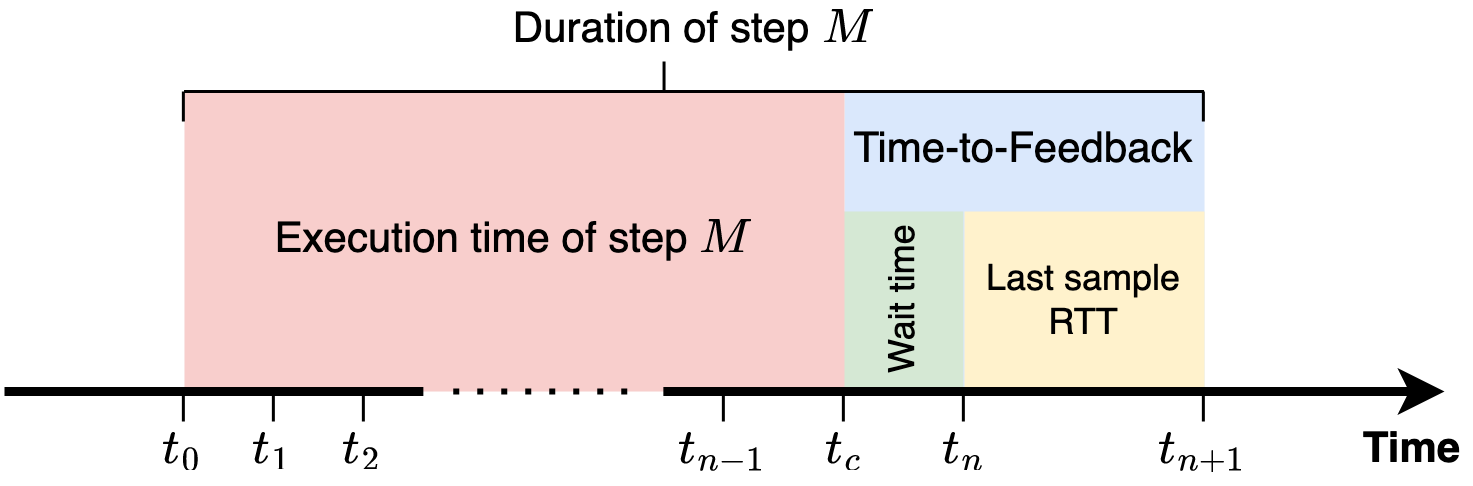
\includegraphics[width=.9\textwidth]{publications/2023EdgeDroid2/figs/step_time}
    \caption[]{%
        Breakdown of a step in a \gls{WCA} into its timing components.
        \ensuremath{t_k | k \in \{1, \ldots, n \}} correspond to sampling instants.
        \ensuremath{t_0} indicates the instant at which the instruction for step \ensuremath{M} is provided to the user and the first sample for said step is captured.
        The instruction for step \ensuremath{M + 1} is provided at \ensuremath{t_{n+1}}.
        Finally, \ensuremath{t_c} marks the instant at which the user finishes the instruction, and \ensuremath{t_n} the instant of capture of the first sample after the instruction has been completed;
        this sample therefore also corresponds to the final sample of step \ensuremath{M}.
        Figure originally included in \cref{paper:olguinmunoz2023realistic}.
    }\label{fig:wcastep}
\end{figure}

An important portion of the present thesis deals with the modeling of human behavior for the benchmarking of \gls{WCA}.
We focus in particular on \emph{step-based} \gls{WCA}, i.e.\ assistance applications which have as their goal the guidance of a user through a task, using a series of instructions.
In this section, we will provide some definitions relating to the operation of these applications.

As discussed above, \glspl{WCA} track the state of the real world through sampling of inputs, most commonly of video feeds.
In step-based \glspl{WCA}, the state in question refers to the progress of some arbitrary, sequential task, such as the assembly of a LEGO model or of a piece of IKEA furniture~\cite{chen2018application}.
We will formally define \emph{task} as a well-defined sequence of instructions to be performed in order to achieve a final goal state, and further define a \emph{step} within a task as a specific action to be performed by the user, described by a single instruction.
A step begins when the corresponding instruction is provided to the user, and ends when the instruction for the next step is provided;
the time interval between these two events will be referred to as the \emph{step duration}.

In the following, please refer to \cref{fig:wcastep}.
\ensuremath{\{ t_0, t_1, \ldots, t_{n + 1} \}} corresponds to a series of discrete and sequential sampling instants, such that \ensuremath{t_0} corresponds to the instant at which the instruction for step \ensuremath{M} is provided and the first sample of the step is taken.
\ensuremath{t_n} corresponds to the instant at which the final sample of step \ensuremath{M} is taken;
this sample is the first sample to capture the finished state of the step.
At this point, the application transitions to the next step \ensuremath{M + 1}, and thus \ensuremath{t_{n + 1}} is the instant at which the next instruction is provided and step \ensuremath{M + 1} begins.
We will also refer to the interval \ensuremath{t_{n + 1} - t_n} as the \emph{last sample \gls{RTT}}.

\glsreset{TTF}%
From this characterization, we can define key variables relating to human behavior with respect to the sampling behavior of these applications.
If we understand \ensuremath{t_c} as the point in time at which the user finishes executing the instruction for step \ensuremath{M}, then
\begin{enumerate*}[itemjoin={{; }}, itemjoin*={{; and }}, label={(\arabic*)}]
    \item \ensuremath{t_c - t_0} corresponds to the \emph{step execution time}, that is, the time it has taken the user to complete the instruction
    \item \ensuremath{t_n - t_c} is the \emph{wait time}, an interval of time during which the task has been finished, but no sample capturing the new state has been taken yet
    \item finally, the interval \ensuremath{t_{n + 1} - t_c} we call \emph{\gls{TTF}}, and refers to the time the user spends waiting for a new instruction.
\end{enumerate*}
These values are key to understanding human perception of responsiveness in these systems, and therefore also to the optimization of resource consumption in \gls{WCA}.
We will refer to them extensively in \cref{chap:contributions}.

%\subsection{Mechanisms relating human behavior to system responsiveness}
%
%The question of how people respond to delay in a computer system is grounded in how people perceive time.
%Time perception has been described as regulated by an attentional gate that, when opened, starts a cognitive pulse counter~\cite{zakay1995attentional,zakay1996role}.
%More recent research indicates, however, that duration perception is highly malleable and the result of multiple timing mechanisms found in overlapping, flexible neural systems~\cite{bruno2016multiple,wiener2011multiple}.
%The estimation of an event's duration varies with context of various types
%\begin{enumerate*}[label={(\roman*)}, before=\unskip{: }, itemjoin={{; }}, itemjoin*={{; and }}]
%\item events subsequent to a long or short interval are contracted or extended, respectively~\cite{heron2012duration}
%\item repeated events tend to be perceived as shorter than novel ones~\cite{matthews2011stimulus}
%\item arousal can expand durations~\cite{droit_volet2011emotion}.
%\end{enumerate*}
%
%Expectations play a critical role in time perception as well~\cite{zakay1995attentional,zakay1996role}.
%It has been shown that people have a general tendency to be hypersensitive to delays in worse-than-expected states, and under-sensitive to meeting or exceeding expectations~\cite{loewenstein1992anomalies}.
%Accordingly, failures to meet expected fast response times tend to be experienced as highly negative, whereas fast latencies are not noticed.
%Violations of expectancy have a strong impact on the acceptability of computer systems.
%Users of a computer system anticipate the latency for events, for which the standards only become more stringent as systems improve in response time.
%In immersive systems like \gls{WCA}, which aim to provide seamless interaction, delays are particularly noticeable.
%
%It has long been recognized that slow system response times can undermine cognitive processing, slow the pace of users, and lead to stereotyped behavior and errors, as well as cause negative emotional consequences~\cite{dabrowski201140}.
%However, standards for what constitute tolerable delays have changed dramatically compared to three decades ago, when delays on the order of \SI{10}{\second} were deemed acceptable~\cite{nielsen1994usability, shneiderman2016designing, seow2008designing}.
%Today's user context, and \gls{WCA} in particular, often demand response times orders of magnitude shorter.
%
%For \gls{WCA} the acceptable range for latencies was explored by Chen et al.~\cite{chen2017empirical}, by constructing assistants for tasks with a range of time constraints, including step-by-step tasks and more interactive contexts like playing Ping-Pong against a human opponent.
%They then proposed a latency tolerance zone according to the task demands.
%For an essentially self-paced task like LEGO assembly, they found two key ranges of latency; unnoticeable, \SIrange{0}{0.6}{\second}; and impaired, \SIrange{0.6}{2.7}{\second}.
%Beyond that, users could begin to show the negative outcomes previously catalogued~\cite{dabrowski201140}.
%
%While behavioral changes and negative interaction outcomes have been well documented in prior research on system delay, the specific mechanisms that mediate these outcomes are less well understood.
%These mechanisms could be cognitive or emotional in origin.
%
%A first possible explanation comes from research on cognitive and motor planning.
%Delay may move users from relatively automatic to more attention-demanding processing.
%Cognitive and motor tasks are commonly described as a hierarchical system, progressing from high-level goals to the sequence of commands that accomplishes them.
%As competency in a task increases, execution of the hierarchy becomes increasingly automated.
%Automatization has been described from a computational perspective in {Anderson's ACT-R}~model as the compiling of multiple productions into one~\cite{neves1981knowledge}.
%Neural measurements indicate that with automaticity, control moves from frontal brain areas to more posterior ones~\cite{jeon2015degree,puttemans2005changes}, and similar distinctions have been related to temporal processing~\cite{lewis2003distinct,koch2009neural,lee2019limiting}.
%
%Although activities guided by a \gls{WCA} are not simple motor actions, immediate feedback after each of a series of repeated actions should promote development and automatic execution of a hierarchical plan.
%Delays, in contrast, would disrupt such a plan through the loss of automated control~\cite{lee2019limiting}.
%
%A second, alternative explanation of delay effects appeals to emotional systems rather than cognitive processes.
%As users of a system become emotionally aroused by delay, they may be subject to generalized arousal, causing decrements in performance~\cite{lee2019limiting}.
%
%Finally, a third potential explanation of delay effects is what has been called ``ego depletion'', the notion that expending effort on self-control eliminates resources needed for further effort~\cite{baumeister74tice,lin2020strong}.
%
%The various processing accounts of delay effects predict different outcomes, which we will consider in the context of the current data.
%If delay increases attentional demands on cognitive processes, responses should be slowed and errors expected, particularly on time-critical tasks.
%Generalized arousal triggered by emotional stress from delay should emerge in physiological measures, such as increased heart rate or skin conductivity.
%Arousal can also reduce movement smoothness or add erratic gestures~\cite{pijpers2003anxiety}.
%Ego depletion has been found to produce premature responses culminating in error~\cite{lin2020strong}, or to lead to abandoning a task entirely~\cite{baumeister74tice}.
%
%Over-arching prescriptions for tolerable system response time have not tended to take into account individual differences in users with respect to salient variables like cognitive ability or personality.
%Relevant research can be found in studies of delay discounting, the tendency to devalue rewards for which one must wait.
%High discounting rates, indicative of waiting intolerance, have been associated with negative social and academic outcomes.
%Hirsh et al.~\cite{hirsh2008delay} found that higher discounting was associated with extraversion among those with low cognitive function, whereas lower discounting was associated with emotional stability (low neuroticism) for people with high cognitive function.
%Among computer system users who tend to have relatively high cognitive ability (which presumably describes the present experimental population), this points to neuroticism as a personality factor that might modulate tolerance for waiting. Extraversion could also  be  a moderating factor among the broader target audience of \gls{WCA}, which are intended for relatively inexperienced users of an application.
%These and other measures of individual variation were considered here.

\subsection{\glsfmtshortpl{NCS} and other \glsfmtshortpl{CPS}}

The number and applications of \glspl{CPS}~\cite{Rajkumar2010CPS} --- i.e.\ systems in which a real, physical mechanism is controlled by a computer --- have exploded in recent years.
However, this rapid increase in adoption has mostly been limited to industrial contexts.
Although \glspl{CPS} present huge opportunities for all facets of society, they have yet to reach our daily lives in any relevant scale due to their stringent operational requirements.
This is about to change, however, as with the advent of novel wireless communication technologies as well as networking paradigms, such as cellular 5G and edge computing~\cite{Satya2017Emergence}, consumer-grade \glspl{CPS} will be made possible.
These technologies meet two key requirements of \glspl{CPS}: real-time capabilities (through extremely low end-to-end latencies), and context- and locality-awareness, and will most likely become the backbone of \gls{CPS} in the future.

\glspl{NCS}~\cite{Gupta2010NCSOverview}, a type of \gls{CPS} wherein multiple networked actuators and sensors form a part of the same automatic control system will benefit from the adoption of these technologies.
Depending on the physical system being controlled, \glspl{NCS} can have stringent timing and reliability requirements for communication that conventional cloud paradigms and cellular networks cannot meet~\cite{Wan2020Efficient}.
This necessitates sophisticated tools for the performance evaluation of future system architectures, as well as novel NCS design paradigm.

%Due to their potential advantages for industrial and commercial settings, there exist works~\cite{Zhang2016Survey} dedicated to the modelling and performance characterization of \glspl{NCS}, improving NCSs by distributing control functions across networks, facilitating centralized coordination, control, and monitoring.

One the one hand, related literature in \glspl{NCS} leverages to a large extent theoretical models, at the price of being able to capture networked systems effects only on a coarse level.
%follows a theoretical approach, and only a small fraction of it deals with experimental studies.
On the other, there exist several approaches when considering experimental methodologies.
%A number of works concerning \glspl{NCS} deal with experimental studies.
%\glspl{NCS} have an inherently inter-domain nature intertwining knowledge from the fields of communications, computing, and control theory in ways that cannot be studied in isolation, leading to various different approaches to such studies.
One such approach uses setups in which the complete system is built on top of real hardware.
This approach is employed in the works of Baumann \emph{et al.}~\cite{Baumann2018LowPower} and Cuenca \emph{et al.}~\cite{Cuenca2019UAV}; in both of these, the authors implement their approach on physical testbeds.
Conversely, other studies choose to instead use completely \emph{simulated} \gls{NCS} setups.
The authors in\ \cite{Ma2019DynamicSched} have opted for such an approach.
These studies often employ combinations of physical and network simulation tools trying to capture the complex dynamics of \glspl{NCS}.
Finally, some experimental studies instead employ \emph{virtualized} approaches, in which either
\begin{enumerate*}[itemjoin={{; }}, itemjoin*={{; or }}]
    \item a real network interacts with a simulated or emulated control system~\cite{Wang2020VoltageControl}
    \item a simulated network interacts with a real control system~\cite{Natale2004InvPendEthernet}.
\end{enumerate*}

As evidenced above, experimental research in \glspl{NCS} includes varied heterogeneous hardware and software platforms, methodologies and key performance indicators.
This, in turn, leads to hardware, software, and methodology fragmentation, as different studies tend to prefer approaches more favored in their respective communities.
Furthermore, existing studies tend to focus on individual aspects and components of a system, thus producing results which do not provide a complete image of the \gls{NCS}.
This has caused a gap in knowledge pertaining to the reproducibility and comparison of experimental studies on these systems.

Zoppi \emph{et al.}~\cite{Zoppi2020NCSBench} made the first (and to the best of our knowledge, the only) attempt at tackling this challenge in their work.
In their work, they proposed a platform called NCSBench, to be used for reproducible benchmarking in NCS.\
Their methodology utilizes joint knowledge of control, computation, and communication.
In their work various architectural elements and the corresponding delays associated with the NCS are modelled.
Multiple experimental parameters and certain observable key performance indicators are defined and utilized in the implementation.
This work however utilizes a physical LEGO\textregistered{}\ Mindstorms EV3 Core Set\texttrademark{}\  based plant for the implementation, preventing instantaneous changes in plant characteristics and component parametrizations.
Furthermore, relying on physical objects like an inverted pendulum limits scalability of the experimentation in practice.

\subsubsection{Benchmarking tools for edge computing}

Experimental research in the area of wireless networking has received ever increasing attention over the last years, driven, on the one hand, by the complexity of modern networked systems and corresponding applications.
On the other, networked systems are more and more based on software instead of dedicated hardware, which allows experimental testbeds to be rededicated simply through an update as system versions evolve --- in contrast to the redeployment of hardware necessitated \numrange[range-phrase={--}]{10}{15} years ago.
The complexity of these systems, as well as their softwarization are expected to continue growing, driving in turn an expanding interest in testbed-based experimental research in wireless systems.

Over the last years, several small- to mid-scale testbeds have emerged that leverage a large degree of freedom with respect to hardware and software, for example, the
\begin{enumerate*}[itemjoin={{, }}, itemjoin*={{, and }}]
    \item \gls{COSMOS}
    \item \gls{POWDER}
    \item \gls{ARA}
    \item Drexel Grid \gls{SDR}
\end{enumerate*} testbeds.
\gls{COSMOS} is a testbed spanning an area of roughly \num{1} square mile (\SI{2.6}{\kilo\meter\squared}) featuring \glspl{SDR}, \si{\milli\meter}-wave equipment, optical fibers, cloud integration, and compute for core network functionality and application data processing~\cite{Cosmos1,cosmos2}.
It contains over \num{200} rooftop, intermediate, and mobile nodes, and is controlled and managed by a central node.
\gls{COSMOS} relies on the \gls{OMF} (originally developed for ORBIT~\cite{orbit}), and employs the \gls{OEDL}, a domain-specific imperative language based on Ruby, for experiment development and definition.

\gls{POWDER} promises research on wireless and mobile networks with a level of programmability down to the waveform~\cite{powder}.
The testbed spans a \SI{15}{\kilo\meter\squared} area and features about \num{15} fixed programmable radio nodes, based on off-the-shelves \glspl{SDR} and featuring edge-like compute capabilities and integration with cloud resources, which interact with \num{50} mobile nodes.
\gls{POWDER} experiments are defined and developed in \emph{profiles}, which correspond to \gls{VM} images containing the necessary software and configurations.
These profiles are defined through using \gls{RSpec}\footnote{\url{https://groups.geni.net/geni/wiki/GENIExperimenter/RSpecs}} documents.

The \gls{ARA} platform is an at-scale testbed for wireless research spanning a rural area with a diameter of over \SI{60}{\kilo\meter} in Iowa~\cite{zhang2022ara}.
Its core goal is the study and deployment of advanced wireless platforms and technologies in real-world agricultural and rural settings.
It includes a broad range of wireless platforms ranging from low-\gls{UHF} massive \gls{MIMO} to \unit{\milli\meter}Wave, deployed through both \glspl{SDR} and programmable \gls{COTS} radios, as well as automated ground vehicles, cameras and sensors.
\gls{ARA}'s software stack, ARASoft, is based upon the highly flexible and powerful \gls{CHI} software suite from the Chameleon testbed project~\cite{keahey2020lessons}, which in turn is based on the widely adopted OpenStack~\cite{openstack} cloud-computing framework.
This affords the \gls{ARA} testbed a high degree of flexibility, as well as lowers the learning curve for new contributors and users.

Finally, the \emph{Drexel Grid \gls{SDR} Testbed} features \glspl{SDR} that connect either over-the-air, through a channel emulator, or over a combination of the two, to facilitate realistic and reproducible experimentation~\cite{DrexelGrid}.
Primarily intended for \gls{SDR}-centric research, it does not integrate any core, cloud or edge components.
However, the testbed extensively employs the \gls{LXC} runtime for the deployment of both experimental code and \gls{SDR} software, which affords users great freedom when it comes to the development of experiments.

Experimentation is key to to fully understanding the implications of next-generation wireless systems, cloud, and edge computing paradigms, and thus more of these testbeds are sure to emerge in the near future.
Yet, little work has so far been devoted to general-purpose, hardware-agnostic software frameworks for the management and automation of such systems.
Existing platforms implement their own, ad-hoc software solutions which are not compatible with other testbeds, and in many cases are not even compatible with reigning cloud-native standards.
This is, for instance, the case with \gls{COSMOS} and \gls{POWDER}; their reliance on domain-specific languages limits their integration with cloud-native solutions, which generally build upon general-purpose languages such as Python and Go.
These testbeds further leverage virtualization technology based on \glspl{VM} instead of more lightweight and edge-compatible solutions such as containers.

To the best of our knowledge, CloudRAFT~\cite{cloudraft} is the only work to tackle (to a certain extent) this challenge.
CloudRAFT corresponds to a cloud-based framework for mobile network experimentation, with a focus on simplifying the management of testbed resources.
The goal of this project is to integrate, coordinate, share, and improve upon existing testbeds; and employs pre-built \glspl{VM} containing the necessary software for experiments.
Although it provides some automation for testbed resource provisioning and experiment execution, its focus is largely rather on the sharing and partitioning of testbed systems.
Testbeds currently working with CloudRAFT include a variety of domain-specific setups, including \pgls{SDR}-based testbed as a well as a ground vehicular robot for mobility-related experimentation.
